\chapter{Shortest Paths}
Ajur picked up a map of the cemetery,  trying to find a way to go to the water fountain. Then he remembered his recent discussions with Rishnak and excitedly told Jura that using Graph Theory methods, they may be able to find a path and even the shortest path. Rishnak was watching Ajur looking at the map and realized that discussion of path and shortest path (length of the path from source vertex to the destination vertex) would be an ideal topic to pursue next.

Consider a graph\footnote{In the case of spanning trees, we consider only undirected graphs; however, for shortest paths we can consider both undirected and directed graphs.}. Rishnak asked Ajur to find the shortest path from a specified source vertex to a specified destination vertex. Consider the following Graph shown in Figure \ref{12g1}.
\begin{figure}
\begin{center}
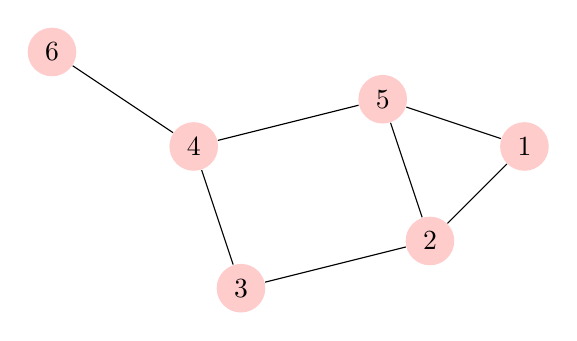
\begin{tikzpicture}
  [scale=.6,auto=left,every node/.style={circle,fill=red!20}]
  \node (n6) at (1,10) {6};
  \node (n4) at (4,8)  {4};
  \node (n5) at (8,9)  {5};
  \node (n1) at (11,8) {1};
  \node (n2) at (9,6)  {2};
  \node (n3) at (5,5)  {3};

  \foreach \from/\to in {n6/n4,n4/n5,n5/n1,n1/n2,n2/n5,n2/n3,n3/n4}
    \draw (\from) -- (\to);

\end{tikzpicture}
\caption{ Example Graph, We want to find the shortest path from vertex 1 to vertex 6}\label{12g1}
\end{center}
\end{figure}

Ajur jumped up and down with excitement and said he could draw the shortest path from source vertex (1) to destination vertex (6) and drew the following graph \ref{12g2}.

\begin{figure}
\begin{center}
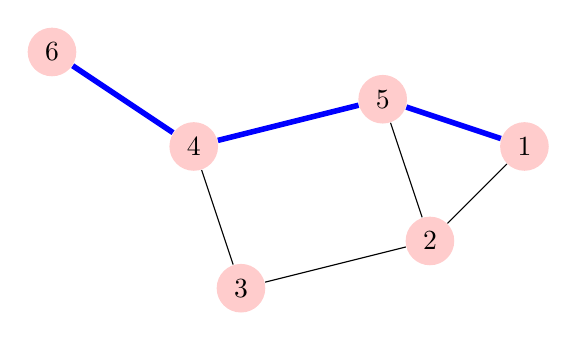
\begin{tikzpicture}
  [scale=.6,auto=left,every node/.style={circle,fill=red!20}]
  \node (n6) at (1,10) {6};
  \node (n4) at (4,8)  {4};
  \node (n5) at (8,9)  {5};
  \node (n1) at (11,8) {1};
  \node (n2) at (9,6)  {2};
  \node (n3) at (5,5)  {3};

  \foreach \from/\to in {n6/n4,n4/n5,n5/n1}
    \draw [line width=2 pt,color=blue] (\from) -- (\to);
\foreach \from/\to in {n3/n4,n3/n2,n2/n1,n2/n5}
    \draw  (\from) -- (\to);

\end{tikzpicture}
\caption{ Example Graph, Shortest Path (of length 3) from vertex 1 to vertex 6 in Graph \ref{12g1} - shortest path is drawn in thick lines.}\label{12g2}
\end{center}
\end{figure}

Pleased with Ajur's enthusiasm, Rishank wanted to make sure Ajur could find a general method for finding the shortest path from a source vertex to a destination vertex.

Rishnak suggested the following method, similar to that of finding any spanning tree \ref{12a1}.

\begin{figure} 
\begin{enumerate}
\item  Label of a vertex, $y$ gives the distance from the source vertex to the vertex $y$.  Let the label \textbf{dist} of the source vertex be 0. The distance from the source vertex to itself is 0. Set label of all the other vertices as unlabeled. Start from the source vertex. Include that vertex in a queue.\footnote{ In a queue, you can only insert in the rear and delete from the front.} 
\item Remove the vertex from the front of the queue. Find all vertices $v$, (not yet labeled) that are adjacent to the removed vertex ($w$) in the queue. Let the label \textbf{dist} of all these vertices be one more than the label \textbf{dist} of $w$ . For each of the newly labeled vertices, set its parent vertex to be $w$ and insert all these vertices in the queue.
\item Repeat the above step till the destination vertex gets labeled with a \textbf{dist} label. We can trace the shortest path starting from the destination vertex and its parent vertex, till we reach the source vertex.
\end{enumerate}
\caption{Finding a shortest Path from source vertex to a sink vertex.}\label{12a1}
\end{figure}

Following the example in Figure \ref{12g1}, let the \textbf{dist} of 1 be 0. Insert 1 in the queue. Delete 1 from the queue. Its (vertex 1) adjacent vertices are 2 and 5. Label the \textbf{dist} of 2 and 5 to be 2. Insert 2 and 5 in the queue. Parent of 2 and 5 are set  to 1. Delete 5 from the queue. Insert the only unlabeled vertex 4 in the queue. Let the label \textbf{dist} of vertex 4 be 2 and let the parent of 4 be 5. The first element in the queue is 2. Delete 2 from the queue. Insert the only unlabeled vertex 3 in the queue.  Let the label \textbf{dist} of vertex 3 be 2 (one more than the \textbf(dist) of 2) and the parent of 3 to be 2. The first element in the queue is 4. Delete 4 from the queue. Insert the only unlabeled vertex 6 in the queue. Let the label \textbf{dist} of 6 be 3 and the parent of 6 be 4. Since 6 is the destination vertex the algorithm stops. The distance from 1 to 6 is 3 and the path is 6, parent(6)=4, parent(4)=5, parent(5)=1 the source vertex.

Ajur marveled at the systematic procedure that could be applied to any graph. He also realized that this procedure could be used to find the shortest path from a single source to all other vertices in a graph and also shortest path between every pair of vertices. Rishnak added that there is a graph parameter called \textbf{diameter} which is the longest path of the shortest path between every pair of vertices. For the example graph shown in \ref{12g2}, the diameter is 3 (as the shortest paths are of lengths 1, 2 and 3). Finding Ajur's eyes glazed, Rishnak asked him to find the diameter for the following graph \ref{12g3}.  

\begin{figure}
\begin{center}
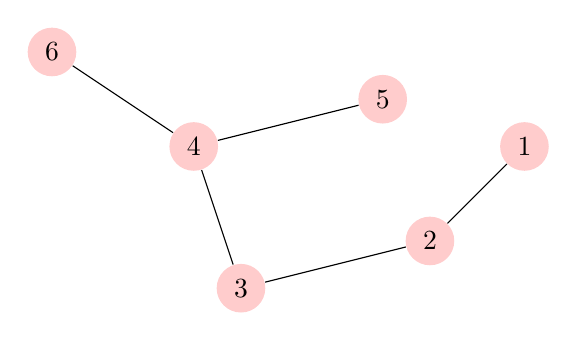
\begin{tikzpicture}
  [scale=.6,auto=left,every node/.style={circle,fill=red!20}]
  \node (n6) at (1,10) {6};
  \node (n4) at (4,8)  {4};
  \node (n5) at (8,9)  {5};
  \node (n1) at (11,8) {1};
  \node (n2) at (9,6)  {2};
  \node (n3) at (5,5)  {3};
   
  \foreach \from/\to in {n6/n4,n4/n5,n1/n2,n2/n3,n3/n4}
    \draw (\from) -- (\to);

\end{tikzpicture}
\caption{ Example Graph, for which we We want to find the diameter }\label{12g3}
\end{center}
\end{figure}

Ajur said that this is the graph \ref{12g1} but with two edges (1,5) and (2,5) are removed. Further, Ajur mentioned it is a tree (as there are no cycles in the graph. The longest path among the shortest paths is from vertex 1 to vertex 5 or from vertex 1 to vertex 6. Both of them are of length 4. Diameter of this graph \ref{12g3} is 4. Ajur mentioned that a simple path with $n$ vertices as shown in Figure \ref{12g4}, the diameter is $n$-1.

\begin{figure}
\begin{center}
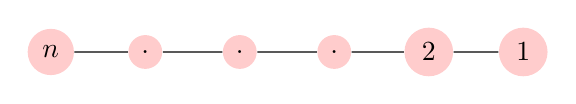
\begin{tikzpicture}
  [scale=.6,auto=left,every node/.style={circle,fill=red!20}]
  \node (n1) at (1,8) {$n$};
  \node (n2) at (3,8)  {$.$};
  \node (n3) at (5,8)  {$.$};
  \node (n4) at (7,8) {$.$};
  \node (n5) at (9,8)  {2};
  \node (n6) at (11,8)  {1};
   
  \foreach \from/\to in {n1/n2,n2/n3,n3/n4,n4/n5,n5/n6}
    \draw (\from) -- (\to);

\end{tikzpicture}
\caption{ A path graph with n vertices whose diameter is $n-1$ }\label{12g4}
\end{center}
\end{figure}

For a complete graph with $n$ vertices the diameter is 1, as the shortest path between every pair of vertices is 1 (as there is an edge between every pair of vertices in a complete graph). 

Rishnak aksed Ajur if he knew how to construct graphs with diameters $n-1, n-1, \cdots, 2, 1$. Ajur repliiied that it was not hard and added that he would show two graphs one with diameter $n-2$ and the other with diameter 2. From there you could infer that he knew all the answers and drew two figures \ref{12g5} and \ref{12g6}.
\begin{figure}
\begin{center}
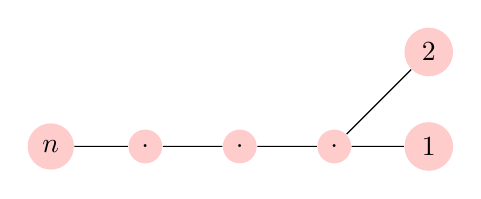
\begin{tikzpicture}
  [scale=.6,auto=left,every node/.style={circle,fill=red!20}]
  \node (n1) at (1,8) {$n$};
  \node (n2) at (3,8)  {$.$};
  \node (n3) at (5,8)  {$.$};
  \node (n4) at (7,8) {$.$};
  \node (n5) at (9,10)  {2};
  \node (n6) at (9,8)  {1};
   
  \foreach \from/\to in {n1/n2,n2/n3,n3/n4,n4/n5,n4/n6}
    \draw (\from) -- (\to);

\end{tikzpicture}
\caption{ A graph with n vertices whose diameter is $n-2$ }\label{12g5}
\end{center}
\end{figure}
\begin{figure}
 \begin{center}
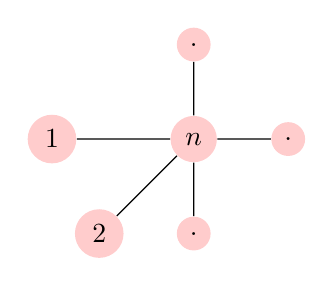
\begin{tikzpicture}
  [scale=.6,auto=left,every node/.style={circle,fill=red!20}]
  \node (n1) at (1,8) {$n$};
  \node (n2) at (1,10)  {$.$};
  \node (n3) at (3,8)  {$.$};
  \node (n4) at (1,6) {$.$};
  \node (n5) at (-1,6)  {2};
  \node (n6) at (-2,8)  {1};
   
  \foreach \from/\to in {n1/n2,n1/n3,n1/n4,n1/n5,n1/n6}
    \draw (\from) -- (\to);

\end{tikzpicture}
\caption{ A graph with n vertices whose diameter is $2$ }\label{12g6}
\end{center}
\end{figure}

Rishnak told Ajur about an interesting problem, that is to construct regular graphs with a given diameter. $k$, $d$ with a number of vertices = $$1+\Sigma_{i=1}^{i=k-1} (d-1)^i$$  Such graphs are called Moore graphs. That formula can be understood by taking a rooted tree of depth $k-1$ with a root vertex has $d$ children and every other vertex has $d-1$ children. All the leaf vertices (vertices of degree 1 in the rooted tree) are connected in such a way that every vertex has degree $d$ and diameter is $k$. (It is no longer a tree). An example of a Moore graph is the Petersen Graph \ref{5g4} and is drawn as a rooted tree with leaf vertices connected Figure \ref{12g7}.
\begin{figure}
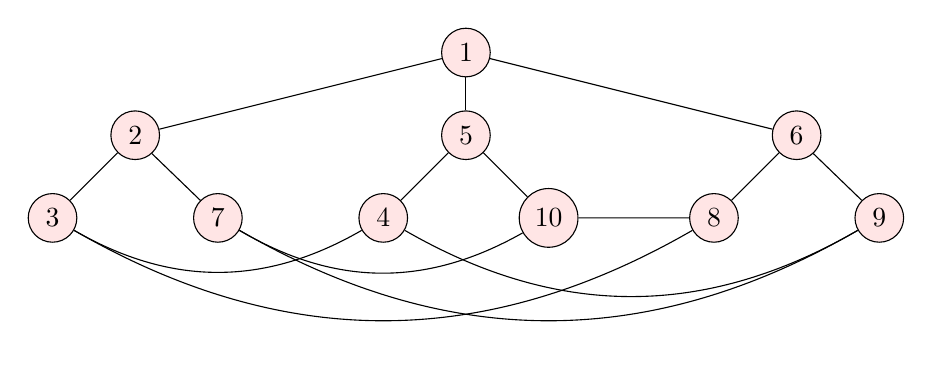
\begin{tikzpicture}[scale=0.7, every node/.style={circle,fill=red!10},level/.style={sibling distance=60mm/#1}]
\node [circle,draw] (z){$1$}
  child {node [circle,draw] (a) {$2$}
    child {node [circle,draw] (b) {$3$}}
    child {node [circle,draw] (c) {$7$}}}
    child {node [circle,draw] (d) {$5$}
        child {node [circle,draw] (e) {$4$}}
        child {node [circle,draw] (f) {$10$}}}
    child {node [circle,draw] (g) {$6$}
        child {node [circle,draw] (h) {$8$}}
        child {node [circle,draw] (i) {$9$}}};
\path
(b) edge [bend right] (h)
(b) edge [bend right] (e)
(c) edge [bend right] (i)
(c) edge [bend right] (f)
(e) edge [bend right] (i)
(f) edge (h)
;
\end{tikzpicture}
\caption{ Petersen Graph drawn as a rooted tree - Its diameter is 2 and it is a regular graph of degree 3 - Same one as in Figure  \ref{5g4}}\label{12g7}
\end{figure}



Ajur then wanted to know there was an algorithm to find the shortest path in a weighted graph.\footnote{Recollect a weighted graph is a graph with weights on edges.} An example weighted graph is shown in Figure \ref{12g8}.
We can modify the algorithm \ref{12a1} for weighted graphs.

\begin{figure} 
\begin{enumerate}
\item  Label of a vertex,$y$ gives the distance from the source vertex to the vertex $y$.  Let the label \textbf{dist} of the source vertex as 0. The distance from the source vertex to itself is 0. Set label \textbf{dist} all the other vertices as $\infty$. Start from the source vertex. Include that vertex in a queue. \footnote{ In a queue, you can only insert in the rear and delete from the front.} Set label \textbf{explored} of the source as 1 and set the \textbf{explored} of other vertices as 0.
\item Remove the vertex from the front of the queue. find all vertices $v$, (for which \textbf{explored} label is 0) that is adjacent to the removed vertex ($w$) in. Let the label \textbf{dist} of all these vertices be minimum of the \textbf{dist} label of $v$ and weight of the edge(w,v)+label \textbf{dist} of $w$ .  Set the parent label of $v$ to $w$ if coming from $w$ is shorter.Among all vertices whose \textbf{explored} label is 0, choose a vertex $w$ whose \textbf{dist} label is the smallest. Set \textbf{explored} of $w$ to 1 and insert $w$ in the queue.
\item Repeat the above step till the destination vertex gets labeled with a \textbf{dist} label. We can trace the shortest path starting from the destination vertex and its parent vertex, till we reach the source vertex.
\end{enumerate}
\caption{Finding a shortest Path from source vertex to a sink vertex.}\label{12a2}
\end{figure}

\begin{figure}
\begin{center}
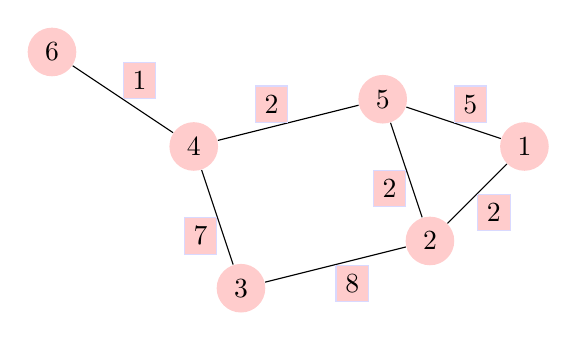
\begin{tikzpicture}
  [scale=.6,auto=left,every node/.style={circle,fill=red!20}]
  \tikzstyle{weight} = [draw=blue!15,shape=rectangle]
  \node (n6) at (1,10) {6};
  \node (n4) at (4,8)  {4};
  \node (n5) at (8,9)  {5};
  \node (n1) at (11,8) {1};
  \node (n2) at (9,6)  {2};
  \node (n3) at (5,5)  {3};
  \foreach \source /\dest /\weight in {n6/n4/1,n4/n5/2,n5/n1/5,n1/n2/2,n2/n5/2,n2/n3/8,n3/n4/7} 
   \draw (\source) --node[weight] {$\weight$}  (\dest);
\foreach \source /\dest /\weight in {1/3/1} place \weight above of=\path;
  
  \end{tikzpicture}
\caption{ Example weighted Graph with 6 vertices and 7 edges - weights are associated with edges. Find the shortest path from vertex 1 to vertex 6.}\label{12g8}
\end{center}
\end{figure}

Using the algorithm described in \ref{12a2} on the Figure \ref{12g8} we get the following.
Initially \textbf{dist} of 1 is 0 and the rest of the vertices it is $\infty$. \textbf{explore} of 1 is 1 and the rest of the vertices it is 0. \textbf{dist} 5 gets 5 and \textbf{2} gets 2. The labels of parent of 2 gets 1 and parent of 5 gets 1. Then \textbf{explore} 2 gets 1. Then \textbf{5} gets 4 and textbf{3} gets 10 and their parent labels become 2. Now \textbf{explore} of 5 is 1. The label \textbf{dist} of 4 becomes 6 and parent label of 4 becomes 5. The \textbf{explore} of 4 is 1. The \textbf{dist} of 6 becomes 7 and its parent node becomes 4. Note that the label \textbf{dist} of 3 and the parent node of 3 does not get affected. Bow \textbf{explore} of 6 becomes 1 and since it is the destination vertex the algorithm stops. The shortest distance between vertex 1 and vertex is 7 and the shortest path can be traced as 6, parent (6)=4, parent (4)=5, parent of 5=2,parent of 2=1 , the source vertex.
Rishnak drew the following figure \ref{12g9} to illustrate the path.

\begin{figure}
\begin{center}
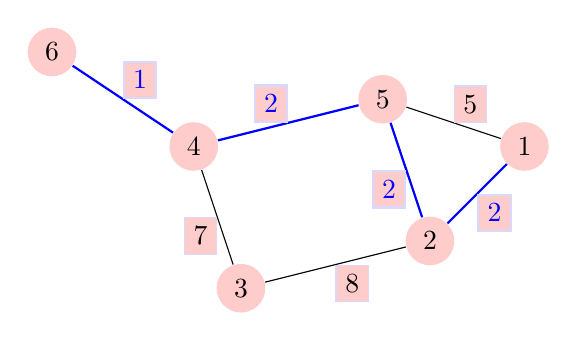
\begin{tikzpicture}
  [scale=.6,auto=left,every node/.style={circle,fill=red!20}]
  \tikzstyle{weight} = [draw=blue!15,shape=rectangle]
  \node (n6) at (1,10) {6};
  \node (n4) at (4,8)  {4};
  \node (n5) at (8,9)  {5};
  \node (n1) at (11,8) {1};
  \node (n2) at (9,6)  {2};
  \node (n3) at (5,5)  {3};
  \foreach \source /\dest /\weight in {n5/n1/5,n2/n3/8,n3/n4/7} 
   \draw (\source) --node[weight] {$\weight$}  (\dest);
\foreach \source /\dest /\weight in {1/3/1} place \weight above of=\path;
  \foreach \source /\dest /\weight in {n6/n4/1,n4/n5/2,n1/n2/2,n2/n5/2} 
   \draw[color=blue,thick] (\source) --node[weight] {$\weight$}  (\dest); 
  \end{tikzpicture}
\caption{ Example weighted Graph with 6 vertices and 7 edges - weights are associated with edges. The shortest path from vertex 1 to vertex 6 is shown.}\label{12g9}
\end{center}
\end{figure}

Ajur appreciated the power of the algorithm, He had seen people using different routes to go from one place to the other. This algorithm may have been used to compute the shortest routes. However, he was getting tired and now wanted to find a shortest path to a bench so he could lie down so along with Jura, drifted off in that direction.